\section{Results}
\label{sec:Results}
In this section we describe the results of our methodologies on the observational and treatment data. We investigate the relations between features and symptoms of the real data provided in the files\footnote{See GitHub} and determine answers to our questions from the data. 

\subsection{Observational Data: Task $1_a$}
\label{subsec:1_a_real}
\graphicspath{{pictures/task1a/}}
In this subsection we use the real data provided in the \textit{Observation-feature.csv} file. 

%Methodology 1, observational data
Applying methodology\textsubscript{1} to the observational data, we obtain the following correlations between features and $Death$ shown in Figure \textbf{Figure \ref{fig:1a1r}}. We firstly observe that vaccines have relevant negative correlations, while for positive correlations $CovidPositive$ is the major influencer of $Death$.

\begin{figure}[H]
  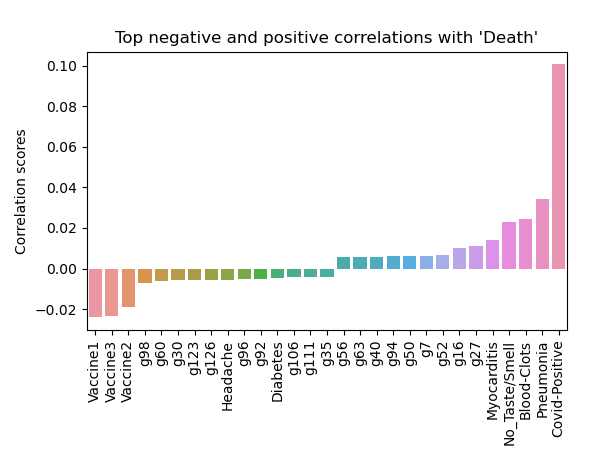
\includegraphics[width=\linewidth]{1a1r.png}
  \caption{Correlations between Death and other features for Observational Data.}
    \label{fig:1a1r}
\end{figure}

\begin{figure}[H]
  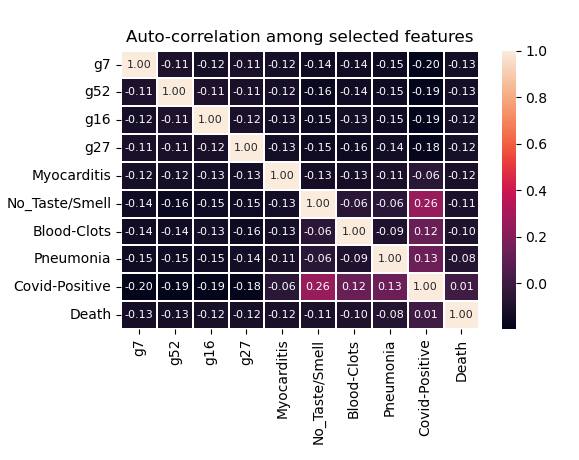
\includegraphics[width=\linewidth]{1a2r.png}
  \caption{Auto-correlations among features for Observational Data.}
  \label{fig:1a2r}
\end{figure}

The auto-correlation matrix in \textbf{Figure \ref{fig:1a2r}} shows high values of correlation between $CovidPositive$ and some symptoms: such as $No\_Taste/Smell$, $Pneumonia$ and $Blood\_Clots$. Hence, similarly to the synthetic data we found that it is necessary to work in a subset of the data containing only the $CovidPositive$ individuals to eliminate the dependence of symptoms on it. As our experiments with synthetic showed, this should allow us to determine the features which are actually predictive of death.

\begin{figure}[H]
  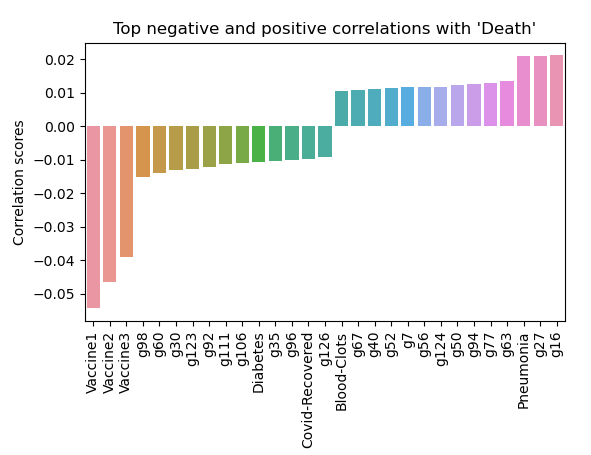
\includegraphics[width=\linewidth]{1a3r.png}
  \caption{Correlations between Death and selected features for Observational Data.}
    \label{fig:1a3r}
\end{figure}
Then we obtain the following correlations, where we can observe that vaccines are much more strongly predictive of survival. Perhaps even more notably, the features most predictive of death are no longer dominated solely by symptoms, but now show several genes which are especially predictive of death, namely $Gene_{16}$, $Gene_{27}$, $Gene_{63}$, $Gene_{77}$ in the top 5 features. The only symptom remaining among the top 5 predictive features was $Pneumonia$.

%Methodology 2, observational data 1a
Following from the useful indications from methodology\textsubscript{1}, we then use methodology\textsubscript{2}, yielding the conditional probability of death given explanatory features.

\begin{figure}[H]
  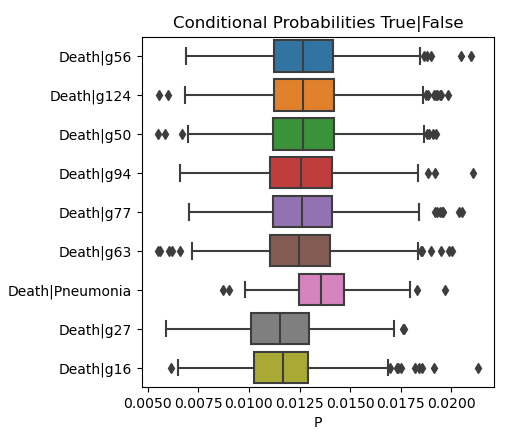
\includegraphics[width=\linewidth]{1a7r.png}
  \caption{Conditional Probability of Death given $Feature = 0$.}
    \label{fig:1a7r}
\end{figure}

\begin{figure}[H]
  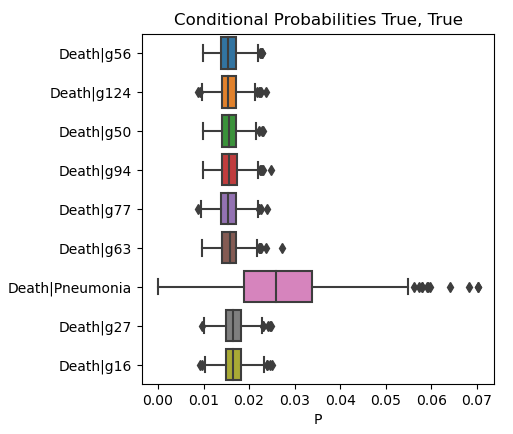
\includegraphics[width=\linewidth]{1a8r.png}
  \caption{Conditional Probability of Death given $Feature = 1$.}
    \label{fig:1a8r}
\end{figure}

\textbf{Figures \ref{fig:1a7r}} and \textbf{\ref{fig:1a8r}} show the conditional probability of death given the features from the dataset. We see in the plots that the probability of death increased by the greatest amount when conditioned on $Pneumonia$, from a mean of approximately $0.013$ to $0.025$. We also see a small increase in the probability of death when conditioned on the gene features, however the range of values when the genes are present versus not present overlap quite heavily. In this regard, we are not able to deduce that these genes affect the probability of death from methodology\textsubscript{2}.

%Methodology 3, observational data 1a

We then apply our final methodology to the observational data to determine our final conclusions with respect to the effect of genes and symptoms on death in the observational data.

\begin{figure}[H]
  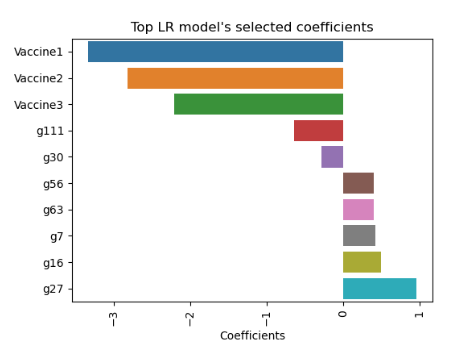
\includegraphics[width=\linewidth]{1a9r.png}
  \caption{Coefficient Values of Logistic Regression observational data, after randomized grid-search 500-fold CV.}
    \label{fig:1a9r}
\end{figure}

\begin{figure}[H]
  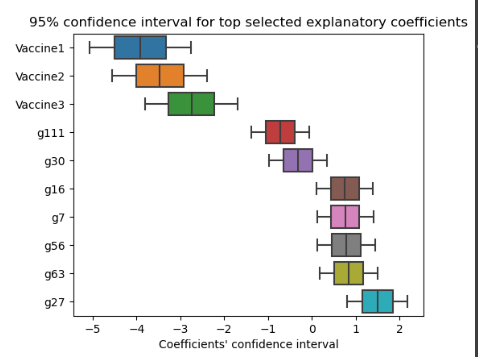
\includegraphics[width=\linewidth]{1a10r.png}
  \caption{95\%  Confidence  Interval  for  Logistic  Regression Coefficient Values.}
    \label{fig:1a10r}
\end{figure}

Following our procedure, the $Logistic$ $regression$ models were trained on the top 10 negatively correlated and top 10 positively correlated features from observational data. When trained with all features, including $CovidPositive$, the logistic regression models were unable to predict $Death$ at any better than $0.5$ (i.e. random guess). When the models were trained on a subset containing only the $CovidPositive$ population without feature selection, the best model had an accuracy of $0.71$. Finally, when using the 10 most negatively and 10 most positively correlated features, the best scoring model had an accuracy of $0.87$. This approach therefore remains the same in our subsequent tasks and models trained for methodology\textsubscript{3}.

The resulting coefficient values are as shown in \ref{fig:1a9r}, with $95\%$ confidence intervals for the logistic regression shown in \textbf{Figure \ref{fig:1a10r}}. This is to say that we are $95\%$ confident that the true value of the coefficient will be within the intervals shown in the figure. From this, we can conclude that if a feature has a lower range of possible values, then it is less predictive of death (or more predictive of death if the range is higher than other features). 

Based on these results along with the previous methodologies, we return to our first set of questions:

\begin{itemize}
    \item \textit{Can we predict death rate given age, gender, income, genes and comorbidities?} 
The logistic regression coefficients and accuracy show that it is possible to train a model which is able to accurately predict death.

    \item Our second question (\textit{Which explanatory features are best to predict death?})
is answered by these results as well, showing that the symptoms and comorbidities which are most effective in predicting death are $Gene_{16}$, $Gene_{63}$ and $Gene_{27}$. $Pneumonia$ did not arise in methodology\textsubscript{3} as a top predictor of death, and $Gene_7$ does not appear from methodologies $1$ and $2$, so we conclude that these features are most likely comparatively less important predictors of death (though likely still risk factors).
\end{itemize}
 
\subsection{Observational Data: Task $1_b, 1_c$}
In this section we apply our methodologies for estimating the efficacy of vaccines and investigate their possible side-effects. The results of methodology 1 are the same as from Subsection \ref{subsec:1_a_real}, but in this case we focus on the fact that each of the vaccines are highly negatively correlated to death (\textbf{Figure \ref{fig:1a3r}}), indicating that they are possibly effective in preventing it.

%Methodology 2, observational 1bc

On the other hand, methodology\textsubscript{2} differs from our previous analysis, as in this case we are modelling the conditional probability of side-effects (including death) from vaccines.
\graphicspath{{pictures/task1b/}}
\begin{figure}[H]
  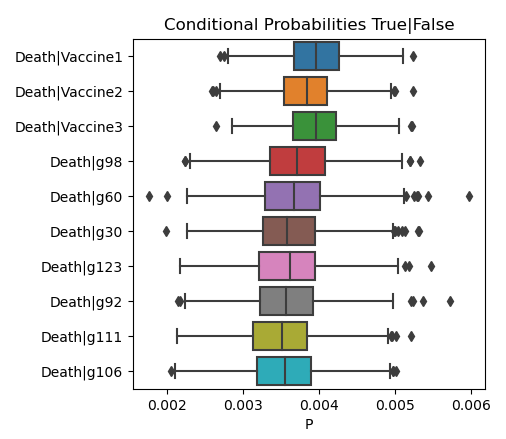
\includegraphics[width=\linewidth]{1b5r.png}
  \caption{Conditional  Probability  of  Death  given $Feature = 0$.}
    \label{fig:1b5r}
\end{figure}

\begin{figure}[H]
  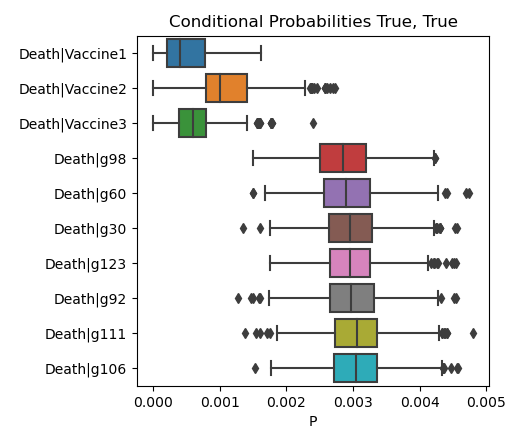
\includegraphics[width=\linewidth]{1b6r.png}
  \caption{Conditional  Probability  of  Death  given $Feature = 1$.}
    \label{fig:1b6r}
\end{figure}

\textbf{Figures \ref{fig:1b5r}} and \textbf{\ref{fig:1b6r}} show the conditional probabilities of side-effects where the patient is unvaccinated and vaccinated, respectively. The figures show that the probability of $Death$ is greatly reduced when conditioned on all of the vaccines, with $Vaccine1$ being the most effective (specifically, reducing the probability of death the most). In this case we also observe that the quantiles for the probability of death given vaccines are greatly below the probability of death without vaccines. Interestingly, while both this methodology and methodology\textsubscript{1} show $Vaccine1$ to have the greatest effect on reducing the probability of death, they differ on which of $Vaccine2$ or $Vaccine3$ is the second most effective in preventing death.

An additional aspect of our analysis with methodology\textsubscript{2} is the estimation of side effects from vaccines. With this methodology we are also able to calculate the conditional probability of symptoms given vaccines. \textbf{Figures \ref{fig:1c3r}} and \textbf{\ref{fig:1c4r}} show that the probability of $Fever$ and $Headache$ symptoms was greatly increased when conditioned on the vaccines. Without vaccines the mean probability of $Headache$ was $0.03$ and $Fever$ was $0.05$. $0.05$ for headache, $0.085$ for Fever. We did not find a similar association with any other side-effects.

The mean probability of $Headache$ symptom increased from approximately $0.03$ to $0.05$ when conditioned on each of the vaccines (all resulted in similar mean values), while the mean probability of $Fever$ increased from $0.05$ to $0.085$. For the probability of $Fever$ and $Headache$ conditioned on each of the vaccines, the quantiles of the probability estimate did not overlap with the probability estimate conditioned on not receiving the vaccine. For this reason we conclude that this is a reasonable indication that the vaccines are associated with $Fever$ and $Headache$ as side effects.

\graphicspath{{pictures/task1c/}}
\begin{figure}[H]
  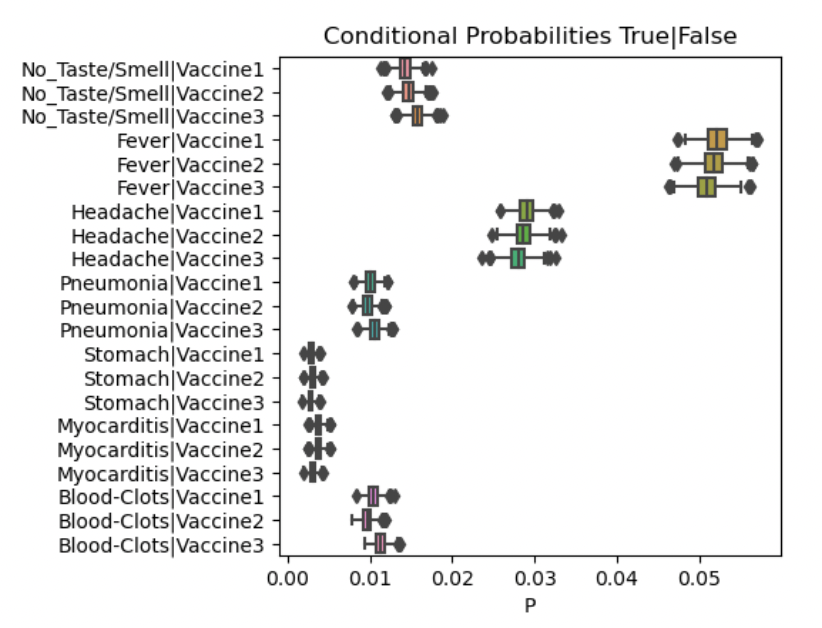
\includegraphics[width=\linewidth]{1c3r.png}
  \caption{Conditional  Probability  of  Symptoms  given $Vaccines = 0$.}
    \label{fig:1c3r}
\end{figure}

\begin{figure}[H]
  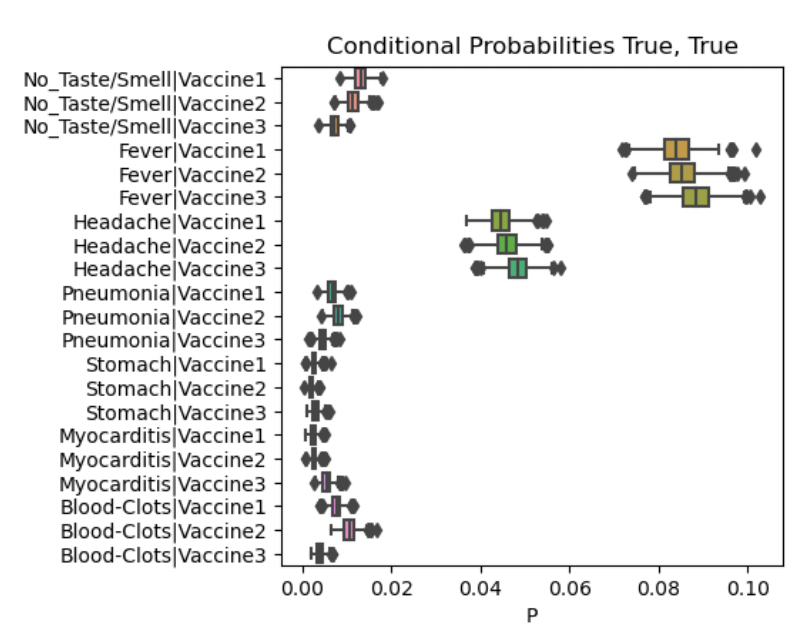
\includegraphics[width=\linewidth]{1c4r.png}
  \caption{Conditional  Probability  of  Symptoms  given $Vaccines = 1$.}
    \label{fig:1c4r}
\end{figure}

%Methodology 3, observational 1bc

Next, turning to methodology\textsubscript{3}, we train $Logistic$ $regression$ models predicting symptoms including death. As with methodology\textsubscript{1}, we refer to the same models described in \ref{subsec:1_a_real} to determine the answer to our second set of questions (Tasks 1b and 1c). The top 3 negative features in the logistic regression model are the three vaccines (\textbf{Figure} \ref{fig:1a9r}), indicating that they are the most predictive of survival. The order of greatest effectiveness can be loosely observed as $Vaccine1$, $Vaccine2$, $Vaccine3$. This  Nonetheless, the confidence intervals on the effectiveness of each vaccine (as measured with the coefficient values) broadly overlap (\textbf{Figure \ref{fig:1a10r}}) and all three can be considered "effective" under this measure (and there may be no reason for a patient to, for instance, prefer $Vaccine1$ to $Vaccine3$ in practice). 

%Side effects here

In conclusion with this, we answer the questions posed for Tasks 1b and 1c. 
\begin{itemize}
\item \textit{Can we predict death rate (efficacy) of a vaccine?}
Yes, our methodologies indicate that all three vaccines are very effective in reducing the chance of death in the Covid-Positive population.

\item \textit{Which vaccine is most effective?}
Our analysis indicates that $Vaccine1$ is the most effective of the three. However, we cannot definitively say whether $Vaccine2$ or $Vaccine3$ is superior, as the results of our methodologies differ on which is more predictive of survival.

\item \textit{Can we predict a specific symptom(s) (side-effect(s)) of a vaccine?}
Through analyzing the conditional probability estimates obtained in methodology\textsubscript{2}, we predict that all three of the vaccines in the data are associated with side-effects of $Headache$ and $Fever$. In the case of features such as blood clots, the conditional probability estimates do not differ sufficiently from the conditional probability of death without the vaccines to conclude that the vaccines may cause them as side effects. Blood clots may be associated with $Vaccine2$ as shown in \ref{fig:1c4r}, but the overlap between this estimate and the baseline is too great to rule out the possibility of this being merely random chance.

\item \textit{Which side-effect(s) each vaccine produce?}
From our analysis it appears that all three vaccines produce $Fever$ and $Headache$ as side-effects, with the unconfirmed possibility of blood clots from $Vaccine3$, as noted above.
\end{itemize}
\subsection{Treatment Data: Task $2$}
\graphicspath{{pictures/task2/}}
In the final subsection we use the real data contained in the files 'treatment\_features.csv', 'treatment\_action.csv' and 'treatment\_outcome.csv' regarding the treatments. 

%Methodology 1, treatment data (Task 2)
We again perform methodology\textsubscript{1} in order to obtain the correlations of features in the data. The results shown in \textbf{Figure \ref{fig:2_1r}} are similar to those in the observational data, with the new addition of $Treatment2$ as a variable which is highly negatively correlated with death. Notably, we do not observe $Treatment1$ in the top 10 negatively correlated variables.

\begin{figure}[H]
  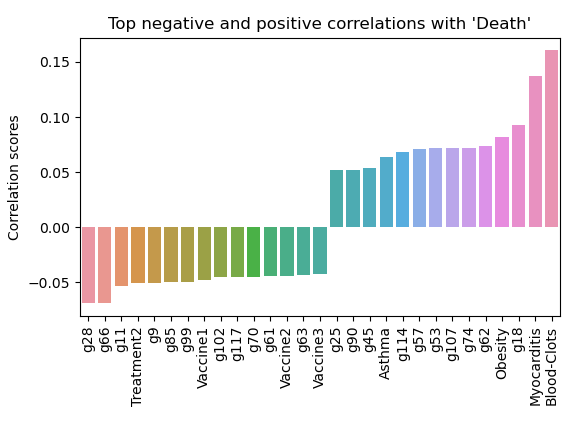
\includegraphics[width=\linewidth]{2_1r.png}
  \caption{Correlations between Death and selected features for Observational Data.}
    \label{fig:2_1r}
\end{figure}

% Methodology 2, treatment data (Task 2)

We then proceed with analyzing \textbf{Figures \ref{fig:2_5r_top}} and \textbf{Figures \ref{fig:2_6r_top}} using methodology\textsubscript{2}. The results show that the probability of $Death$ conditioned on $Treatment2$ appears to be lowered, but there is some overlap in the estimates from this method. For this reason, these results may not be as indicative in establishing that $Treatment2$ is effective in preventing $Death$. 

\begin{figure}[H]
  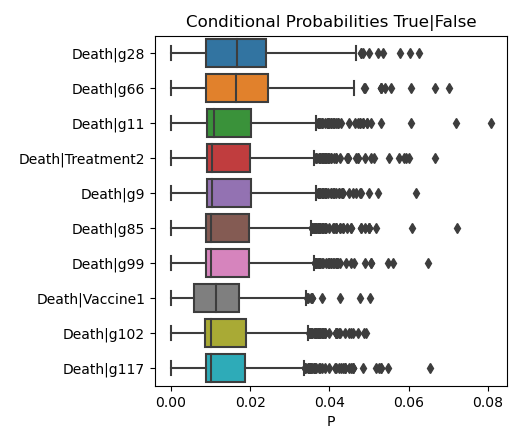
\includegraphics[width=\linewidth]{2_5r_top.png}
  \caption{Conditional Probability of $Death$ given selected $Features = 0$.}
    \label{fig:2_5r_top}
\end{figure}
\begin{figure}[H]
  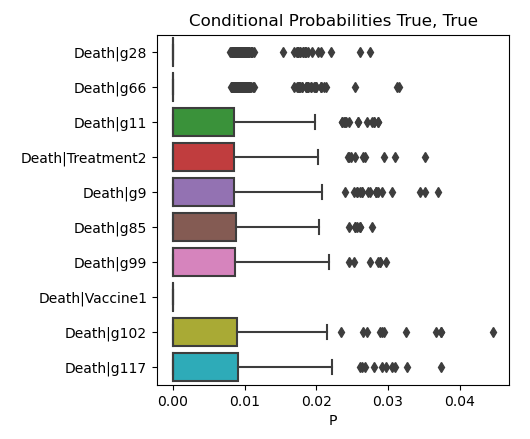
\includegraphics[width=\linewidth]{2_6r_top.png}
  \caption{Conditional Probability of $Death$ given selected $Features = 1$.}
    \label{fig:2_6r_top}
\end{figure}

We also observe in \textbf{Figures \ref{fig:2_5r_after}} and \textbf{\ref{fig:2_6r_after}} that the probability of symptoms when conditioned on treatments are very similar to the probability when conditioned on the absence of treatment. The one notable feature of these charts is that the probability of $Blood\_clots$ conditioned on $Treatment 1$ is $0$. This is however a very marginal result and so we can not establish any evidence of side-effects from treatments using this method. We note that the amount of total samples in the data was very small, particularly with respect to certain symptoms. This may be a reason that this methodology does not reach a clear conclusion and estimates several probabilities precisely at $0$.

\begin{figure}[H]
  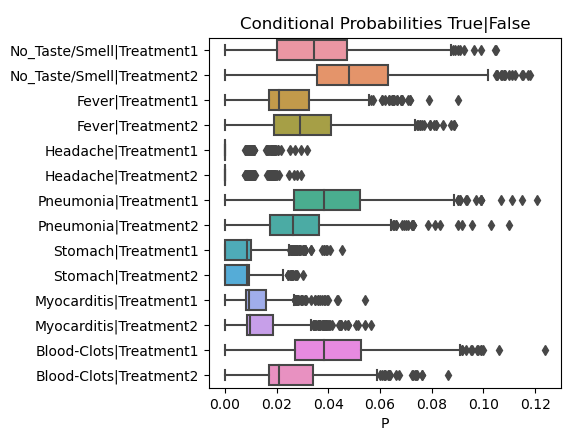
\includegraphics[width=\linewidth]{2_5r_after.png}
  \caption{Conditional Probability of Symptoms given $Treatments = 0$.}
    \label{fig:2_5r_after}
\end{figure}
\begin{figure}[H]
  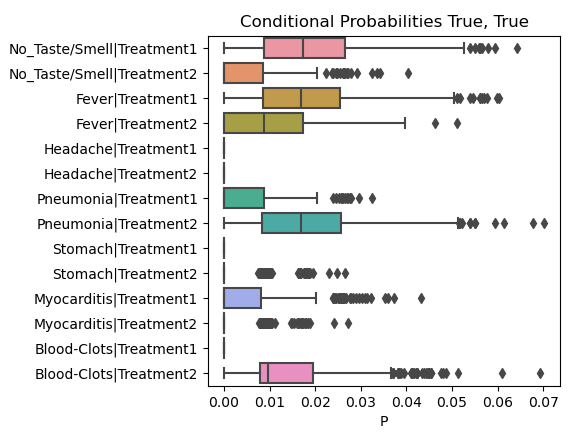
\includegraphics[width=\linewidth]{2_6r_after.png}
  \caption{Conditional Probability of Symptoms given $Treatments = 1$.}
    \label{fig:2_6r_after}
\end{figure}

%Methodology 3, treatment data (Task 2)

Our last analysis of the treatment data is performed with methodology\textsubscript{3}. In this case, due to the scarcity of data points, we train the $Logistic$ $regression$ model using bootstrapping to re-sample the data, in order to balance the outcomes for the training process. The resulting best model accuracy is $0.98$ with confidence intervals as in \textbf{Figure \ref{fig:2_12r}}. We observe once again in \textbf{Figure \ref{fig:2_11r}} that the the coefficient for $Treatment1$ is not in the top selected features. On the other hand, $Treatment2$ is once again among the most negatively associated variables with $Death$. Combined with our observation from methodology\textsubscript{1}, this indicates that $Treatment2$ is effective at preventing $Death$, and very likely more effective than $Treatment1$.

\begin{figure}[H]
  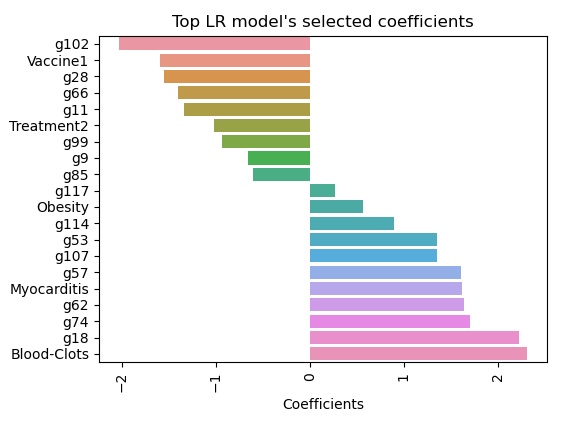
\includegraphics[width=\linewidth]{2_11r.png}
  \caption{Coefficient Values of Logistic Regression, after randomized grid-search 500-fold CV.}
    \label{fig:2_11r}
\end{figure}

\begin{figure}[H]
  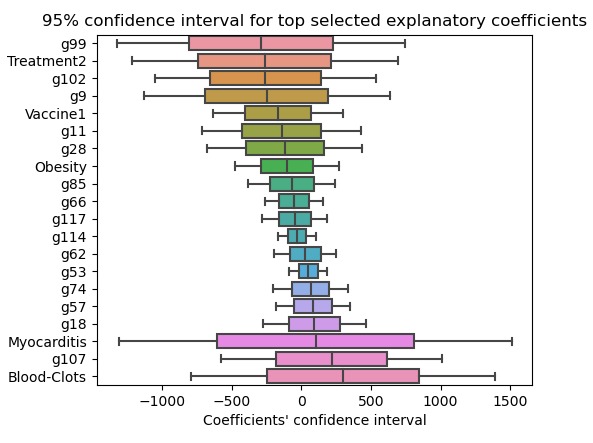
\includegraphics[width=\linewidth]{2_12r.png}
  \caption{95\%  Confidence  Intervals  for  Logistic  Regression Coefficient Values.}
    \label{fig:2_12r}
\end{figure}

We are then able to answer the questions we posed for Task 2.

\begin{itemize}
\item \textit{Can we predict death rate given a specific treatment?}
Yes, we are able to train a logistic regression model which is able to predict death among the $CovidPositive$ population with an cross-validated accuracy of $0.98$. 
\item \textit{Which treatment is the most effective?}
We estimate that the probability of death for a patient given $Treatment2$ is lower than without treatment, as well as lower than when given $Treatment1$. While $Treatment1$ may still be effective in preventing death (we do not establish that it is not), our analysis indicates that $Treatment2$ is more effective.
\item \textit{Can  we  predict  a  precise  symptom(s)(side-effect(s))  given  a  specific  treatment?}
We were not able to establish that any side-effects were more likely given either of the treatments. We speculate that this may be due to the low number of samples for each symptom, such that our calculation of conditional probabilities was not able to make an precise estimate approximating the actual outcomes.
\item \textit{Which side-effect(s) does each treatment produce?}
As noted in the previous answer, we cannot establish any side-effects from the treatments, and conversely we also do not establish that the treatments do \textbf{not} cause side effects.
\end{itemize}